%----------------------------------------------------------
%----------------------------------------------------------
% MARCO TEÓRICO

A lo largo del presente capítulo se pretende describir los conceptos en torno a los cuales se efectuará el siguiente trabajo. Además se llevará a cabo una revisión de las  tecnologias relacionadas con este proyecto como  son las  plataformas open hardware, sensores y microcontroladores .\\

%--------------------------------------
\subsection{Open Hardware}
\subsubsection{¿Qué es Open Hardware?}
Se les llama Open Hardware a todos los dispositivos de hardware cuyas especificaciones y diagramas esquemáticos son de acceso público, ya sea bajo algún tipo de pago o de forma gratuita. Algo que tienen en común el Open Hardware y el Open Software es que ambos corresponden a las partes tangibles de un sistema informático.

El Open Software ofrece al usuario cuatro libertades de uso, de estudio  y modificación, de  distribución y de redistribución de las versiones modificadas. Existen licencias que  garantizan y dan cobertura legal,  como  por  ejemplo  la  licencia  GNU GPL. El Open Hardware toma es mismas ideas del Open Software para aplicarlas en su campo.\cite{Osh14}

Esta idea es tan antigua  como la  del Open Software, sin embargo  su  empleo no es tan directo compartir  diseños  de  hardware  es  un poco  más  complicado no se cuenta  con una definición exacta. Incluso Richard Stallman Presidente de la  Free Software Foundation afirma  que  las  ideas del Open Software  se  pueden  aplicar  a los archivos  o fichero necesarios  para el diseño y especificación, pero no  al circuito físico  en  sí.  

Al no existir una  definición clara de Open Software cada persona  lo  interpreta  a su manera. Dependiendo  del  enfoque  pueden  ser  establecidas dos clasificaciones  la primera  tiene en cuenta  cómo es  su naturaleza estático o  reconfigurable  y la  otra   en función  de  su filosofía.

\subsubsection*{Según su Naturaleza}

Dada su diferente naturaleza, al hablar de Open hardware hay que especificar de qué tipo de hardware se está hablando. A continuación se describen cada uno de los diferentes hardwares según su naturaleza:

\begin{itemize}
\item \textbf{Hardware reconfigurables}\\
Es aquél descrito mediante un lenguaje de descripción de hardware. Su naturaleza es completamente diferente a la del hardware estático. Se desarrolla de una manera muy similar a como se hace con el software, mediante archivos de texto, que contienen el código fuente. Se les puede aplicar directamente una licencia libre, como la GPL. Los problemas no surgen por la definición de qué es libre o qué debe cumplir para serlo, sino que aparecen con las herramientas de desarrollo necesarias. Para hacer que el hardware reconfigurable sea libre, sólo hay que aplicar la licencia GPL a su código.\\
\item \textbf{Hardware estático}\\
Es el conjunto de elementos materiales o tangibles de los sistemas electrónicos.
\end{itemize}

\subsubsection*{Según su filosofía}

Al no existir una definición clara de Open Hardware, también existe libertad en su interpretación. Muchos de los argumentos acerca del diseño de Open Hardware provienen de quienes hablan en las comunidades de software y hardware. Una causa de esto es el simple hecho de que la palabra ``software'' refiere tanto al código fuente como a los archivos o ficheros ejecutables, mientras que las palabras ``hardware'' y ``diseño de hardware'' se refieren claramente a dos cosas distintas. Usar la palabra ``hardware'' como taquigrafía para el diseño y el objeto físico es una receta para la confusión. Los términos siguientes se han utilizado en discusiones de este asunto.

\begin{itemize}
\item \textbf{Free hardware design}\\
Se refiere a un diseño que pueda ser copiado, distribuido, modificado, y fabricado libremente. No implica que el diseño no pueda también ser vendido, o que cualquier puesta en práctica de hardware del diseño estará libre de coste. Todas las mismas discusiones sobre el significado de la ``libertad'' entre los partidarios de la \emph{Free Software Foundation}, y los partidarios de la Licencia BSD que afecta al software, desafortunadamente las trasladan a los diseños del hardware.\\
\item \textbf{Open source hardware}\\
Se refiere al hardware para el cual toda la información del diseño se pone a disposición del público en general. Open source hardware se puede basar en un free hardware design, o el diseño en el cual se basa puede ser restringido de alguna manera.\\
\item \textbf{Open Hardware}\\
Es una marca registrada del Open Hardware Specification Program. Es una forma limitada de open source hardware, para la cual el requisito es que: La suficiente documentación del dispositivo debe estar disponible para que un programador competente pueda escribir un controlador del dispositivo. La documentación debe cubrir todas las características de la interfaz del dispositivo - controlador que se espera que cualquier usuario emplee. Esto incluye funciones de entrada-salida, de control y funciones auxiliares como medidas de funcionamiento o diagnósticos de auto prueba. Los detalles de soporte de firmware on-board y de la puesta en práctica de hardware no necesitan ser divulgados excepto cuando son necesarios para permitir programar un controlador para el dispositivo.\cite{Del07}

Es decir, solamente una cantidad de información limitada sobre el diseño necesita estar disponible; posiblemente no mucha, por ejemplo, para hacer una reparación.

\end{itemize}




%--------------------------------------
\subsection{Biometría}

Históricamente, la identificación personal se ha basado en posesiones especiales (llaves, tarjetas) o en conocimientos secretos (palabras claves, números de identificación personal), todos estos aspectos son casi únicos, y se emplean para verificar la identidad de su portador. Ahora bien, el ser humano posee características propias que lo hacen único: huellas dactilares, la voz, el rostro, la forma de escritura, e incluso el iris del ojo.Entonces, podemos decir que nosotros llevamos nuestras propias palabras claves, tarjetas o números PIN. Entonces, ¿Porque no aprovechar estas características?\\

Los científicos se formularon está misma pregunta hace algunos años, dando
origen a la Biometría. Ésta consiste en la identificación o verificación de la identidad de un individuo, empleando sus características biológicas, psicológicas y de conducta. En la actualidad, existen distintos tipos de dispositivos que soportan la biometría, tales como
lectores de huella digital o lectores de retina.\cite{Car08}\\
\newpage

Por definición, un sistema biométrico, es un sistema automático capaz de:\\

\begin{enumerate}

\item Obtener la muestra biométrica del usuario final.
\item Extraer los datos de la muestra.
\item Comparar los datos obtenidos con los existentes en la base de datos.
\item Decidir la correspondencia de datos.
\item Indicar el resultado de la verificación.
\end{enumerate}

Algunos de los dominios para esta tecnologia son:
\begin{itemize}
\item \textbf{Bioinformática}: Aplicación de la informática en el área de la medicina y la biología.
\item \textbf{Biometría forense}: La ciencia y tecnología de usar e interpretar la evidencia física para propósitos legales.
\item \textbf{Interacción Humano-Computador \textit{(Human-to-Computer Interaction-HCI)}}: Su objetivo es mejorar el rendimiento y la precisión de esas interfaces, mediante el reconocimiento de los usuarios y adaptarse a las características específicas de cada usuario para labores de reconocimiento.
\item \textbf{Seguridad biométrica}: Autenticación de usuarios. Enlazar la información digital a una determinada identidad para lograr control de acceso, autenticación de información entre otras.
\end{itemize}

En  este  trabajo de  titulación,este  último dominio es el  que nos interesa y  en el  cual  se  centraremos especial  atención y esfuerzos.

Cabe destacar que todos los métodos biométricos conocidos son ``no determinísticos'' y necesitan estar basadas en aproximaciones heurísticas.

Existen 2 modos de operación en los sistemas de autenticación biométrica: El enrolamiento (\textit{Enrollment}) y la autentificación (\textit{Authentication}).

\subsubsection{Enrrolamiento y Autenticación}


Existen 2 modos de operación en los sistemas de autenticación biométrica: El enrolamiento (\textit{Enrollment}) y la autentificación (\textit{Authentication}).


\subsubsection*{Enrolamiento}

El proceso de enrolamiento ocurre cuando nos registramos en el sistema, donde las características de cada usuario se almacenan para futuras referencias y asociaciones de identidad de los sujetos. Una representación gráfica de este modo se aprecia en la Figura \ref{enrrolamiento}

\begin{figure}[H]
\centering
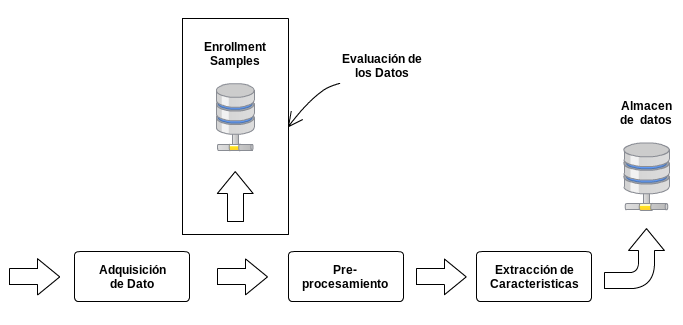
\includegraphics[scale=0.5]{images/capitulo2/enrrolamiento.png}
\caption{Esquema gráfico del proceso  de Enrrolamiento}
\label{enrrolamiento}
\end{figure}

Aquí se observa que el proceso comienza con la toma de datos (por ejemplo, medir y realizar conversiones análogo-digital). La representación digital posterior a este proceso es denominada Enrollment Samples(Ejemplos de Enrolamiento) o simplemente enrollments. Desde el enrollment original se extraen las características biométricas, son preprocesadas, y en algunos casos almacenadas en algún soporte de datos (como una base de datos) para poder reproducirlas en otro momento.

\subsubsection*{Autenticación}

La Autenticación (\textit{authetication}) consiste en el proceso de verificar o identificar la identidad de algún sujeto, según corresponda,  en la Figura \ref{autenticacion} se muestra en forma gráfica este proceso.

\begin{figure}[H]
\centering
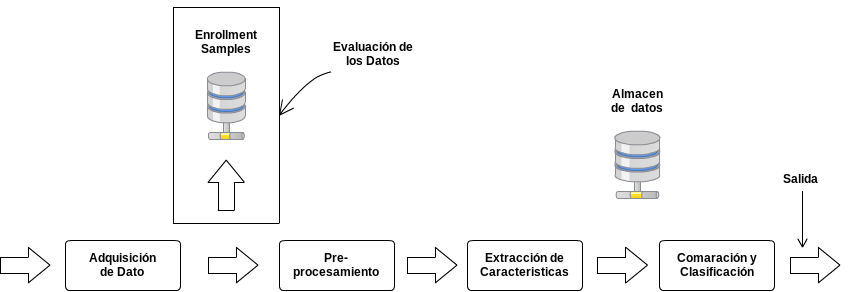
\includegraphics[scale=0.5]{images/capitulo2/autenticacion.png}
\caption{Esquema gráfico del proceso  de Autenticación}
\label{autenticacion}
\end{figure}


\subsubsection{Verificación versus Identificación}

La autenticación la podemos dividir en dos acciones verificación y identificación, en función de cómo se desee obtener la identidad del sujeto.

\subsubsection*{Verificación}
El modo de Verificación es el sistema de autentificación que determina si un set determinado de características son similares al template de dicha persona para determinar si es o no es la persona. El resultado de esta acción es siempre una decisión binaria(si o no, 0 o 1) entregando en algunos casos el puntaje de acierto (Matching Score), lo que muestra el grado de similitud entre su template y ésta persona.

\subsubsection*{Identificación}

El modo de Identificación describe el proceso de determinar la identidad de un sujeto (dadas sus características biométricas) comparándolas con un rango de sujetos. Así, la clasificación asignada será una entre todas las personas registradas en el sistema.



Para ejemplificar estos conceptos, veamos los siguientes ejemplos.

\begin{itemize}

\item Si tenemos un control de acceso para un portal principal, nuestro problema es ``Determinar quién es'', para en función de eso, determinar si ingresa o no. Esto sería una identificación.

\item Si tenemos una oficina del usuario ``Pedro Paredes'', donde sólo él tiene asignado acceso, nuestro problema es ``Determinar si soy Pedro Paredes'', por lo tanto, verificar si soy el usuario determinado. Esto es una verificación.
\end{itemize}

Es fundamental entender ambos mecanismos y encontrar el más adecuado para nuestros requerimientos.

\subsubsection{Criterios de selección de características biométricas}

Se han sugerido distintos criterios para autenticar de manera adecuada. A continuación veremos los 4 más importante:
\begin{enumerate}
\item \textbf{La Variabilidad} La Variabilidad tiene que ver con la variación de los valores desde un evento a otro, sobre una misma persona. Este efecto es llamado variabilidad Intra-Personal o Intra-Class. La variabilidad es inherente a todos los sistemas biométricos debido a la naturaleza no determinística de las mediciones biométricas, en la Figura \ref{la_variabilidad} vemos un ejemplo de variabilidad  \cite{Way00}.\\

\begin{figure}[H]
\centering
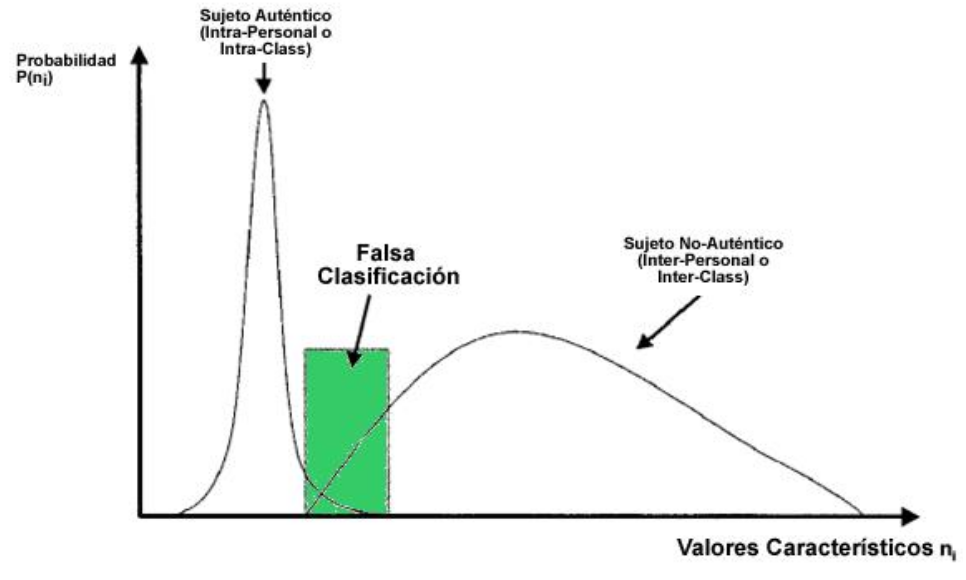
\includegraphics[scale=0.3]{images/capitulo2/la_variabilidad.png}
\caption{Ejemplo de variabilidad y capacidad de discriminar una característica biométrica}
\label{la_variabilidad}
\end{figure}


\item \textbf{La Capacidad Discriminatoria}  está determinada por el grado de unicidad de las características biométricas que serán utilizadas en la comparación. Aparentemente, un buen sistema biométrico posee una baja variabilidad Intra-Personal y una alta variabilidad Inter-Personal (entre distintas personas). El grado de variabilidad Intra-Personal está reflejado por el ancho de una distribución gaussiana (ver Figura \ref{la_variabilidad}) para sujetos auténticos, donde la capacidad discriminatoria puede ser estimada en la intersección de las curvas de sujetos auténticos versus sujetos no-auténticos \cite{Zha00}.\\

\item \textbf{La Acertividad}, para diseñar un sistema biométrico funcional, las características deben poseer bastante acertabilidad en un tiempo aceptable. Hoy en día, el criterio es determinado por la tecnología del sensor, planteando la inquietud de saber si obtuvo la característica en un tiempo aceptable y con la suficiente calidad. Por ejemplo, un examen de ADN es muy exacto, sin embargo, requiere un amplio tiempo de trabajo de verificación \cite{Zha00}.


\item \textbf{El Rendimiento}, cuando nos referimos a que una característica biométrica debe ser procesada en un tiempo aceptable nos referimos al rendimiento de un sistema biométrico.  de una persona para el ingreso a una oficina. Por lo general asociamos el grado de exactitud en función del tiempo de respuesta que deseemos obtener \cite{Way00}.

\end{enumerate}


\subsubsection{Medidas de Rendimiento y Exactitud}

Los sistemas biométricos intentan determinar o verificar la identidad de cada miembro registrado en nuestro sistema utilizando medidas y/o características distintivas. Debido a la naturaleza no-determinística de este proceso, es imposible realizar un análisis exacto (con los sistemas del día de hoy). Evaluaciones técnicas sugieren que éstas deben ser realizadas mediante análisis estadísticos y mediciones empíricas.

Según el tipo de medición biométrica que deseemos utilizar, se utilizan distintos indicadores. A través de las últimas 2 décadas, se llegó al consenso en cuáles eran las mediciones más importantes, para realizar las evaluaciones técnicas pertinentes \cite{Way99} y que son presentadas en la tabla \ref{tabla_medidas}.



\begin{spacing}{1.0}
\begin{table}[H]
\centering
\caption{Pricipales medidas para evaluaciones de los sistemas biométricos} 
\begin{tabular}{|c|c|}
\hline 
\rowcolor{green!50} &\\
\rowcolor{green!50} \textbf{Medida} & \textbf{Descripción}\\[0.3cm]
\hline 
\textbf{Tasa de Falsos Aciertos} &\makebox[8.5cm][l]{Tasa entre coincidencias detectadas por el sistema}\\
\textit{False Match Rate} (FMR)  &\makebox[8.5cm][l]{pero que no son reales (falsos positivos) versus el}\\
\textit{False Accept Rate} (FAR) &\makebox[8.5cm][l]{número total de muestras.}                           \\
\hline
\textbf{Tasa de Falso Rechazo} &\makebox[8,5cm][l]{Tasa entre coincidencias que no son detectadas}\\
\textit{False Non-Match Rate (FNMR)} & \makebox[8,5cm][l]{por el sistema pero que sí son reales (falsos}\\
\textit{False Reject Rate (FRR)} & \makebox[8,5 cm][l]{negativos) versus el número total de muestras.}\\
\hline
\textbf{Tasa donde los errores son iguales} & \makebox[8,5cm][l]{El punto en el diagrama de tasa de errores donde}\\
\textit{Equal-Error-Rate (EER)} & \makebox[8,5cm][l]{las tasa de falsos aciertos es igual a la tasa de}\\
 & \makebox[8,5cm][l]{falsos rechazos.} \\
\hline
\textbf{Tasa de error por particionamiento} & \makebox[8,5cm][l]{Tasa de falsos rechazos debido a errores de}\\
\textit{Binning Error Rate (BNR)} & \makebox[8,5cm][l]{particionamiento.}\\
\hline
\textbf{Coeficiente de Penetración} & \makebox[8,5cm][l]{Porcentaje promedio del tamaño del repositorio}\\
\textit{Penetration Coefficient (PC)} & \makebox[8,5cm][l]{de datos a ser revisado para cada proceso de} \\
 & \makebox[8,5cm][l]{autenticación.}\\
\hline
\textbf{Tiempo de Transacción} & \makebox[8,5cm][l]{Tiempo requerido para una sola transacción de}\\
\textit{Transaction Time (TT)} & \makebox[8,5cm][l]{autenticación, compuesto por la suma del tiempo}\\
 & \makebox[8,5cm][l]{de recolección de datos y el tiempo de cálculo.}\\
\hline

\end{tabular}
\label{tabla_medidas}
\end{table}
\end{spacing}

Las dos primeras medidas definen el umbral de decisión (\textit{threshold}) desde donde  se puede optimizar el nivel de exactitud en función del tiempo de búsqueda como  se muestra en la Figura\ref{umbral}. esto quiere decir que a un alto valor de umbral implica un sistema menos exacto, por lo  cual podria aceptar a quien no posee los permisos correspondientes, pero más rápido a la hora de entregar resultados. Por el contrario, con un bajo umbral de decisión, es menos probable equivocarse, pero el tiempo de procesamiento es mucho mayor. A pesar de la importancia de estos indicadores en los distintos dispositivos biométricos, no es objetivo de este proyecto de título entrar en mayores detalles.


\begin{figure}[H]
\centering
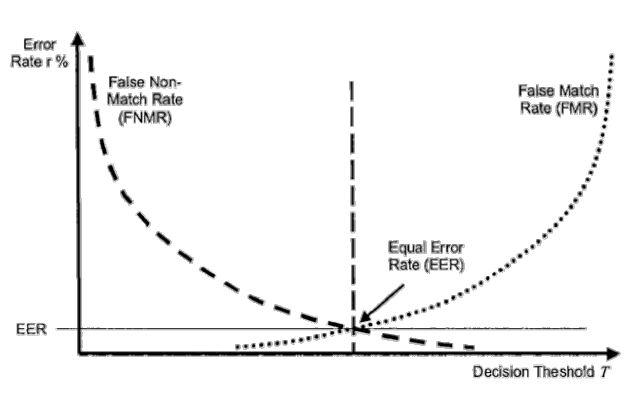
\includegraphics[scale=0.5]{images/capitulo2/umbral.png}
\caption{FNMR, FMR y EER en función del umbral de decisión}
\label{umbral}
\end{figure}

\subsubsection{Dactiloscopía: Reconocimiento de huellas dactilares}

La base de ésta modalidad biométrica es la estructura que posee la piel en la punta de los dedos. Se trata de una característica biológica fenotípica, es decir, una manifestación específica de determinados rasgos, que serían únicos, incluso en caso de personas que son gemelos.\\

La estructura biométrica está compuesta por ``crestas papilares'' y los ``surcos interpapilares'', comúnmente llamados ``crestas'' y ``valles''. Las crestas papilares son los relieves epidérmicos situados en la palma de las manos y en la planta de los pies, mientras que los surcos interpapilares se determinan por las depresiones que separan dichos relieves o crestas. Dentro de las crestas papilares existen los llamados ``poros papilares'', que son diminutos orificios de variadas formas y dimensiones por los cuales se expulsa el sudor. Una vez que el sudor sale al exterior, se derrama por todas las crestas y se mezcla con la grasa natural de la piel, dando lugar a que cuando se toque un objeto apto para la retención de huellas, éstas queden impresas en el mismo. Esta es la base de la impresión dactilar [WIK08a].

%-------------------------------------------------------------------------------------------------------------------------------------------



En la Tabla \ref{tabla_inalambricas} se presenta una clasificación de las diferentes tecnologías de comunicación inalámbricas \cite{Kuo07}, señalando sus principales características  y aplicaciones tPorcentaje promedio del tamaño del repositorioípicas, a fin de observar las condiciones que presenta el 802.15.4, donde se concentrará la atención del presente trabajo.

\begin{spacing}{1.0}
\begin{table}[H]
\centering
\caption{Clasificación de tecnologías de comunicación inalámbricas} 
\begin{tabular}{|c|c|c|c|c|}
\hline 
\rowcolor{gray!30} &&&&\\
\rowcolor{gray!30} \textbf{Clase} & \textbf{Velocidad} & \textbf{Radio de} & \textbf{Aplicaciones} & \textbf{Ejemplo de}\\ 
\rowcolor{gray!30} & \textbf{de datos} & \textbf{cobertura} & \textbf{típicas} & \textbf{tecnologías}\\[0.3cm]
\hline 
&&&&\\[-0.2cm]
WWAN & $<$10 Mbps & $>$10 km & Telefonía, & GSM, UMTS,\\
 & & & Internet móvil, & satélite\\[0.2cm]
\hline 
&&&&\\[-0.2cm]
WMAN & $<$100 Mbps & $<$10 km & Internet & IEEE 802.16,\\
 & & & banda ancha & HIPERMAN\\[0.2cm] 
\hline
&&&&\\[-0.2cm]
WLAN & $<$100 Mbps & $<$100 m & reemplazo LAN & IEEE 802.11,\\
 & & & alámbrica & HIPERLAN/2\\[0.2cm] 
\hline
&&&&\\[-0.2cm]
WPAN & $<$10 Mbps & $<$10 m & transferencia & Bluetooth,\\
 & & & de datos personales & IEEE 802.15.3\\[0.2cm]  
\hline
&&&&\\[-0.2cm]
WSN & $<$1 Mbps & $<$1 km & monitoreo, & redes propietarias,\\
 & & & control & IEEE 802.15.4,\\ 
 & & & & RFID\\[0.2cm] 
\hline
\end{tabular}
\label{tabla_inalambricas}
\end{table}
\end{spacing}

\vspace{0.2cm}

El estándar IEEE 802.15.4 tiene como principales atributos su bajo coste en términos de requerimientos y bajo consumo de energía, destacando en aplicaciones domóticas e industriales. Con una trama que no debe exceder los 127 Bytes de longitud, el estándar ofrece tasas de transmisión de datos de hasta 250 Kb/s, brindando soporte para aplicaciones que no requieran gran velocidad de transmisión, o para nodos alimentados por baterías donde el energía sea un factor crítico. En la Figura \ref{espacio_operacion} se muestra el espacio de operación de los estándares WLAN Y WPAN \cite{Gut04}; cabe destacar que el 802.15.4 no está diseñado para solaparse con estándares de redes inalámbricas de gama alta.

\begin{figure}[H]
\centering
\includegraphics[scale=0.42]{images/capitulo2/espacio_operacion.png}
\caption{Espacio de operación de WPAN y WLAN}
\label{espacio_operacion}
\end{figure}

La Tabla \ref{tabla_comparacionWPAN} \cite{Gut04} presenta un resumen de las principales características de una LR-WPAN (\textit{Low-rate Wireless Personal Area Network}) usando el estándar IEEE 802.15.4, comparado con el estándar IEEE 802.11b y el estándar 802.15.1 (WPAN/Bluetooth).\\

\begin{spacing}{1.0}
\begin{table}[H]
\centering
\caption{Comparación de LR-WPAN con otras tecnologías inalámbricas} 
\begin{tabular}{|>{\columncolor{gray!30}} c| >{\centering\arraybackslash}p{3.1cm}| >{\centering\arraybackslash}p{3.1cm}| >{\centering\arraybackslash}p{3.1cm}|}
\hline 
\rowcolor{gray!30} &&&\\
\rowcolor{gray!30} & \textbf{802.11b} & \textbf{Bluetooth} & \textbf{Low Rate WPAN}\\ 
\rowcolor{gray!30} & \textbf{WLAN} & \textbf{WPAN} & \\[0.3cm]
\hline 
&&&\\[-0.2cm]
\textbf{Rango} & $\sim$100 m & $\sim$10 - 100 m & 10 m\\[0.2cm]
\hline
&&&\\[-0.2cm]
\textbf{Velocidad de datos} & $\sim$2 - 11 Mb/s & 1 Mb/s & $\leq$ 0.25 Mb/s\\[0.2cm]
\hline
&&&\\[-0.2cm]
\textbf{Consumo de energía} & Medio & Bajo & Ultra bajo\\[0.2cm]
\hline 
&&&\\[-0.2cm]
\textbf{Tamaño} & Largo & Pequeño & Pequeñísimo\\[0.2cm]
\hline 
&&&\\[-0.2cm]
\textbf{Costo/Complejidad} & Alto & Medio & Muy bajo\\[0.2cm]
\hline 
\end{tabular}
\label{tabla_comparacionWPAN}
\end{table}
\end{spacing}

Es importante destacar que el 802.15.4 no es sinónimo de la especificación ZigBee, ya que el 802.15.4 es un protocolo de capas Física y de Enlace (capas OSI 1 y 2), mientras que ZigBee es un protocolo de capa de red (capa OSI 3) que se sitúa sobre el IEEE 802.15.4. Además, ZigBee es una marca comercial de la ZigBee Alliance\footnote{\url{http://www.zigbee.org/}}, grupo que crea y mantiene el estándar.\\

De esta forma, es posible manifestar con determinación que la tecnología LR-WPAN busca brindar solución en ámbitos donde una WPAN resulta demasiado costosa y donde se requiere un funcionamiento con un consumo mínimo de energía.\\ 



%----------------------------------------------------------
%----------------------------------------------------------
